\documentclass[a4paper,onecolumn]{article}
\usepackage{amsmath, amsthm, graphicx, amssymb, wrapfig, fullpage, subfigure, array}
\usepackage[font=sl, labelfont={sf}, margin=1cm]{caption}
\DeclareMathOperator{\e}{e}
\begin{document}
\setcounter{page}{1}

\title{Derivation of PoMDP Bellman Equation}
\author{}
\date{}
\maketitle


\section{Notations}
$\mathcal{S}$\quad state space\\
$\mathcal{A}$\quad action space\\
$\mathcal{O}$\quad observation space\\
$\mathcal{B}$\quad belief state space\\
$N$\quad cardinality of $\mathcal{S}$\\
$t$\quad number of time before termination\\
$T$\quad state transition probability,
$\mathcal{S}\times\mathcal{A}\rightarrow \mathbb{R}$, $T(s_{i}, a_i,
s_{i+1}) = \mathbb{P}(s_{i+1}|s_i, a_i)$\\
$R$\quad immediate reward, $\mathcal{S}\times\mathcal{A}\rightarrow
\mathbb{R}$, $R(s_i, a_i)$\\
$\rho$\quad average immediate reward, $\rho(b_i, a_i) =
\sum_{s}b_i(s)R(s, a_i)$\\
$O$\quad observation probability, $O(a_i, s_{i+1}, o_i) =
\mathbb{P}(o_i|a_i, s_{i+1})$, $o_i\in \mathcal{O}$\\
$b$\quad belief state, $b=\{b_1, \cdots, b_N\}$, $b_j =
\mathbb{P}(s=j)$\\
$SE$\quad state estimator, $b_{i+1} = SE(b_i, a_i, o_i)$\\
$V_t(b)$\quad value of being $b$ with $t$ time left\\
$\alpha$\quad $\alpha$-vector, length $N$, $V_t(b) =
\max_k\left(\alpha^k_t\cdot b\right)$. Policy is embedded in $\alpha$.\\
$\tau$\quad belief transition probability, $\tau(b_i, a_i,
b_{i+1}) = \mathbb{P}(b_{i+1}|b_i, a_i)$\\
Notice: $s_i, s_{i+1}$ and $s, s^\prime$ may be used interchangably.

\begin{center}
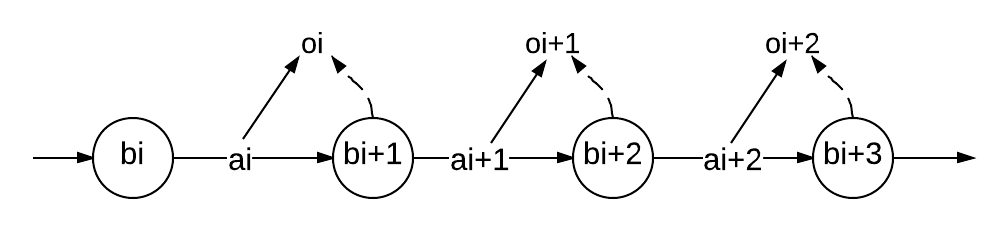
\includegraphics[height=3cm]{beliefMC.png}
\end{center}

\section{Derivation}
\begin{equation}
    V_{t+1}(b) = \max_{a\in\mathcal{A}}\left[\rho(b, a)+ \gamma
	\sum_{b^\prime\in \mathcal{B}}\tau(b, a, b^\prime) V_t(b^\prime)\right]
\end{equation}
Notice, if $b, a, o$ are given, then $b^\prime$ is fixed.
\begin{equation}
    \sum_{b^\prime\in\mathcal{B}} \tau(b, a, b^\prime)V_t(b^\prime) =
	\sum_{o\in\mathcal{O}}
	\mathbb{P}(o|a, b) V_t(SE(b,a,o))
\end{equation}
The $s^\prime$ entry of $SE$ is
\begin{equation}\begin{split}
    SE_{s^\prime}(b,a,o) &= \mathbb{P}(s^\prime|a, o, b)\\
	&=\frac{\mathbb{P}(o|s^\prime, a,
	b)\mathbb{P}(s^\prime|a,b)}{\sum_{s^\prime\in
	\mathcal{S}} \mathbb{P}(o|s^\prime, a,
	    b)\mathbb{P}(s^\prime|a,b)}\\
	&= \frac{
	  O(a,s^\prime, o) \sum_s T(s,a,s^\prime)b(s)
	}{
	  \sum_{s^\prime}O(a,s^\prime, o) \sum_s T(s,a,s^\prime)b(s)
	}
\end{split}\end{equation}
\begin{equation}\begin{split}
    \mathbb{P}(o|a,b) &= \sum_s b(s) \mathbb{P}(o|a,s)\\
	&= \sum_s b(s) \sum_{s^\prime} \mathbb{P}(o,s^\prime|a,s)\\
    &= \sum_s b(s) \sum_{s^\prime}
	\mathbb{P}(s^\prime|a,s)\mathbb{P}(o|a,s^\prime)\\
	&= \sum_s b(s) \sum_{s^\prime} T(s,a,s^\prime)O(a,s^\prime, o)
\end{split}\end{equation}
Let $k = l(b^\prime) = l\left(SE(b,a,o)\right) \equiv l(b,a,o)$ be the $\alpha$-vector
index for $V_t(b^\prime) =
\max_k(\alpha^k_t\cdot b^\prime)$.
Therefore,
\begin{equation}
    V_{t+1}(b) = \max_a\left\{
	  \sum_s b(s)R(s,a) + \gamma \sum_o\left(
	    \sum_s b(s)\sum_{s^\prime} T(s,a,s^\prime) O(a,s^\prime,o)
	  \right)\,
	  \left(\alpha^{l(b,a,o)}_t \cdot SE(b,a,o)\right)
	\right\}
\end{equation}
After simplification,
\begin{equation}
    V_{t+1}(b) = \max_{a\in\mathcal{A}}\left\{
	    \sum_{s\in\mathcal{S}} b(s)
		\underbrace{
		\left(
		  R(s,a) + \gamma \sum_{j=1}^N
		  T(s,a,s_j)
		  \sum_{o\in\mathcal{O}}
		  \alpha_{tj}^{l(b,a,o)}O(a,s_j,o)
		\right)
		}_{Y_s(a,b)}
	\right\}
	\label{Bellman}
\end{equation}

\section{Piecewise Linear Discussion}
$Y_s(a,b)$ is piecewise constant on $b$. Prove as follows,
\begin{center}
    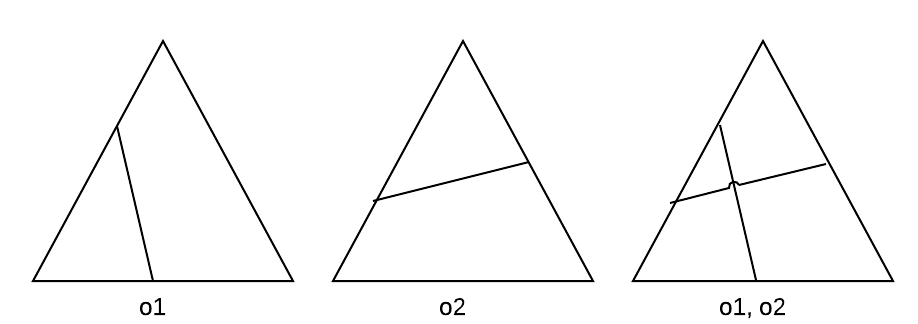
\includegraphics[height=5cm]{partition.png}
\end{center}
These triangles shows $\mathcal{B}$.
Given $a$ and $o$, $l(b,a,o)$ is piecewise constant. For example, given
$a$, $\mathcal{B}$ is partitioned by the value of $l$ into the first
picture given $o_1$, and into the second picture given $o_2$. Given $a$, take the
intersections (refinement) of all partitions of different
$o\in\mathcal{O}$, get the third picture. For this given $a$, within this refined partition,
$l(b,a,o)$ is constant for $\forall o$. So $Y_s(a,b)$ is
piecewise constant in the refined partition. Therefore, $V_{t+1}(b)$ is
piecewise linear. Convexity can also be shown, but the proof is
neglected here.\\

\noindent For a given $a$, it is shown $Y_s(a,b)$ is piecewise constant.
After taking maximum of Eqn\eqref{Bellman}, we have
\begin{equation}
    V_{t+1}(b) = \sum_{s\in\mathcal{S}}b(s) Y^*_s(b)
\end{equation}
$Y^*_s(b)$ is piecewise constant. Its partition includes the intersection
(refinement) of $Y_s(a,b)$ for $\forall a\in \mathcal{A}$ (accounts for
observation change, black lines), and optimal action change (accouts for
change of optimal action, grey lines).
\begin{center}
    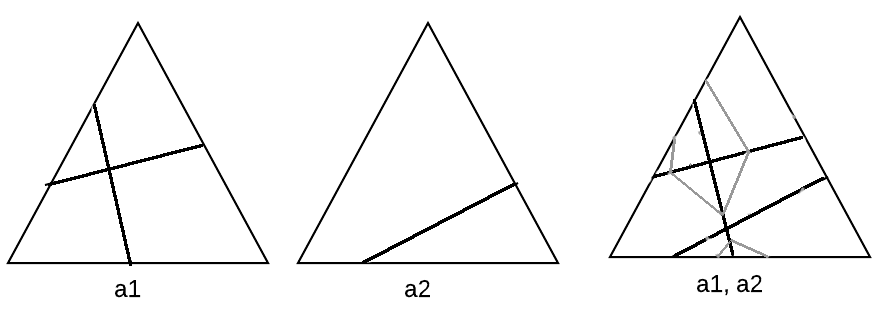
\includegraphics[height=5cm]{partition_a.png}
\end{center}
\subsection{Question}
If we use mesh-based function approximation instead of piecewise linear
(exact) $V(b)$, how to adaptively tweak the mesh (mesh-adaptive)?

\section{Q-Learning in CoMDP}
Q-learning is useful if the agent does not know the form of immediate
reward and state transfer function in the environment.\\
Q-learning maintains a table of Q-values, $Q(s,a)$, that is the
cumulative discounted reward of being in state $s$ and take action $a$.
In the begining the $Q$-value table is estimated, then we update
$Q$-value by
\begin{equation}
    Q_{t+1}(s,a) = r + \gamma \max_{a^\prime} Q_t(s^\prime,a^\prime)
\end{equation}
Here we assume the agent observes $s^\prime$ and $r$ as soon as $a$ is
taken. Note $t$ here means iteration number, not time.\\
The exploration probabilities of taking action $a$ at state $s$ is
chosen by
\begin{equation}
    \mathbb{P}(a|s) = \frac{e^{Q(s,a)\eta}}{\sum_j e^{Q(s,a_j)}\eta}
\end{equation}
\subsection{Question}
How to facilitate $Q$-learning with a non-perfect environment model?\\

\noindent Sometimes, a relaxition can be added to $Q$-learning
\begin{equation}
    Q_{t+1}(s,a) = Q_t(s,a) + \alpha \left(r + \gamma \max_{a^\prime}
	Q_t(s^\prime,a^\prime) -Q_t(s,a)\right)
\end{equation}
$0\le\alpha\le 1$ is the learning rate.

\section{Continuous-state PoMDP}
\noindent In discrete state problem, the belief state is a \emph{point} on 
a hyperplane (a line for two-state problem).
In continous-state problem, the belief state is a distribution on the
state space. For example, if we parameterize states by 2 parameters,
then the state space is a 2D plane. And, a belief state is a
probability distribution (or a normalized function) on the 2D plane.
The $V(b)$ will be a functional that evaluates every possible functions.
The convexity of $V(b)$ indicates: the average of $V$'s for two
probability distributions will be higher than the $V$ for the averaged
probability distribution.\\

\noindent For discrete state, $\alpha$-vector assigns each state a
value, and $V(b) = \max_i <\alpha_i, b>$. In continuous state,
$\alpha_i$ is a function defined on state space, $V(b) = \max_i <\alpha_i, b>$

\end{document}








